\documentclass[11pt,twocolumn]{article}
\usepackage[utf8]{inputenc}
\usepackage[T1]{fontenc}
\usepackage{amsmath,amssymb}
\usepackage{booktabs}
\usepackage{graphicx}
\usepackage[margin=0.75in]{geometry}
\usepackage{hyperref}

\title{\textbf{21cmCU}: A Native C/CUDA and Multi-GPU Accelerated Simulation Engine for 21cmFAST v4}
\author{Haina Huang \and 21cmCU Contributors}
\date{November 2026 (v0.9.0)}

\begin{document}
\maketitle

\begin{abstract}
We present \textbf{21cmCU} (\texttt{py21cmcu} v0.9.0), a native C/CUDA and cuFFT GPU engine with \textbf{86 native CUDA C APIs} compiled directly into the \textbf{21cmFAST v4} CFFI shared library with zero Python GPU wrapper dependencies. Retaining full algorithmic parity with discrete halo models, spin-temperature evolution, \texttt{CLASS} baryon--CDM relative velocities, and lightcone observables, 21cmCU achieves up to \textbf{492.74$\times$} speedup on standalone redshift-space distortions (\texttt{apply\_rsds}), \textbf{82.05$\times$} end-to-end on rectilinear lightcones (3.032\,s vs.\ 248.773\,s on a 16-core CPU), \textbf{71.65$\times$--71.88$\times$} on $256^3$ single-pass interferometer mocks (\texttt{SKA1-Low}/\texttt{HERA-350}), \textbf{20.65$\times$} on \texttt{AngularLightconer}, and \textbf{12.36$\times$} on multi-redshift \texttt{L-INTEGRAL + TS} coeval runs on an NVIDIA GeForce RTX 4090. Through \texttt{v0.7.0--v0.9.0}, 21cmCU adds zero-copy \texttt{\_\_dlpack\_\_} PyTorch streaming (\texttt{OnlineSBIDataset} with warm persistent \texttt{BatchPool}), anti-repetition \texttt{ObliqueRectilinearLightconer} traversal ($12.45\times$ path extension), and CUDA-accelerated 3D bispectrum ($26.64\times$), MFP bubble-size distributions ($62.53\times$--$72.87\times$), exact Minkowski functionals ($8.28\times$--$8.48\times$), CIC particle/galaxy gridding ($39.29\times$ for $1\text{M}$ particles on $256^3$), $21\text{cm} \times \text{galaxy}$ cross-power ($20.68\times$), kSZ momentum maps, and Common-Random-Number (CRN) Fisher forecasting, while scaling multi-GPU slab streaming across $3\times$ RTX 4090 natively in-VRAM to \textbf{$2048^3$ (8.590 billion voxels)} Zel'dovich initial conditions in \textbf{58.467\,s}.
\end{abstract}

\section{Introduction}
Cosmic Dawn and Epoch of Reionization (EoR) 21\,cm intensity mapping experiments such as HERA, LOFAR, and SKA-Low rely on fast three-dimensional semi-numerical simulations for Bayesian MCMC sampling \cite{Mesinger2011,Greig2015,Murray2020} and neural simulation-based inference \cite{Cranmer2020}. With the introduction of discrete halo realizations and richer astrophysical source models in 21cmFAST v4 \cite{Davies2025}, single-node OpenMP runs require several minutes per spin-temperature lightcone, while multi-billion-voxel boxes ($1536^3$--$2048^3$) exceed single-GPU memory capacity.

\textbf{21cmCU} eliminates Python-side GPU framework overhead by embedding CUDA kernels and \texttt{cuFFT} pipelines \cite{cuFFT} directly inside \texttt{c\_21cmfast}, offering drop-in acceleration across single-GPU SBI sweeps and out-of-single-GPU slab-distributed volumes.

\section{Native Architecture and Execution Modes}
At build time (\texttt{USE\_CUDA=1}, \texttt{CUDA\_ARCHS=auto}), \texttt{build\_cffi.py} auto-detects host GPU compute capabilities via \texttt{nvidia-smi} and links CUDA C/cuFFT modules (\texttt{cuda\_mempool.cu}, \texttt{cuda\_ic.cu}, \texttt{cuda\_perturb.cu}, \texttt{cuda\_ionize.cu}, \texttt{cuda\_ts.cu}, \texttt{cuda\_bt.cu}, \texttt{cuda\_lightcone.cu}, \texttt{cuda\_ps.cu}, \texttt{cuda\_io.cu}, and \texttt{cuda\_mgpu.cu}) directly into the CFFI extension alongside 64-bit array indexing.

Users select between two verified modes:
\begin{itemize}
  \item \textbf{\texttt{strict}}: strict IEEE FP32 evaluation matching 16-core CPU reference tolerances.
  \item \textbf{\texttt{fast}}: enables device-resident \texttt{--use\_fast\_math} kernels and fused GPU lightcone/RSD pipelines while remaining calibrated in $\langle x_{\mathrm{HI}} \rangle$, $\langle \delta T_b \rangle$, and 1D/2D power spectra.
\end{itemize}

\section{Single-GPU Speedups, Residency, and I/O}
All benchmarks were captured on cluster node \texttt{b1} (64-core x86\_64 host with \texttt{N\_THREADS=16} for CPU baselines, $1\times$--$3\times$ RTX 4090 24\,GB, CUDA 12.6).

\begin{figure*}[t]
  \centering
  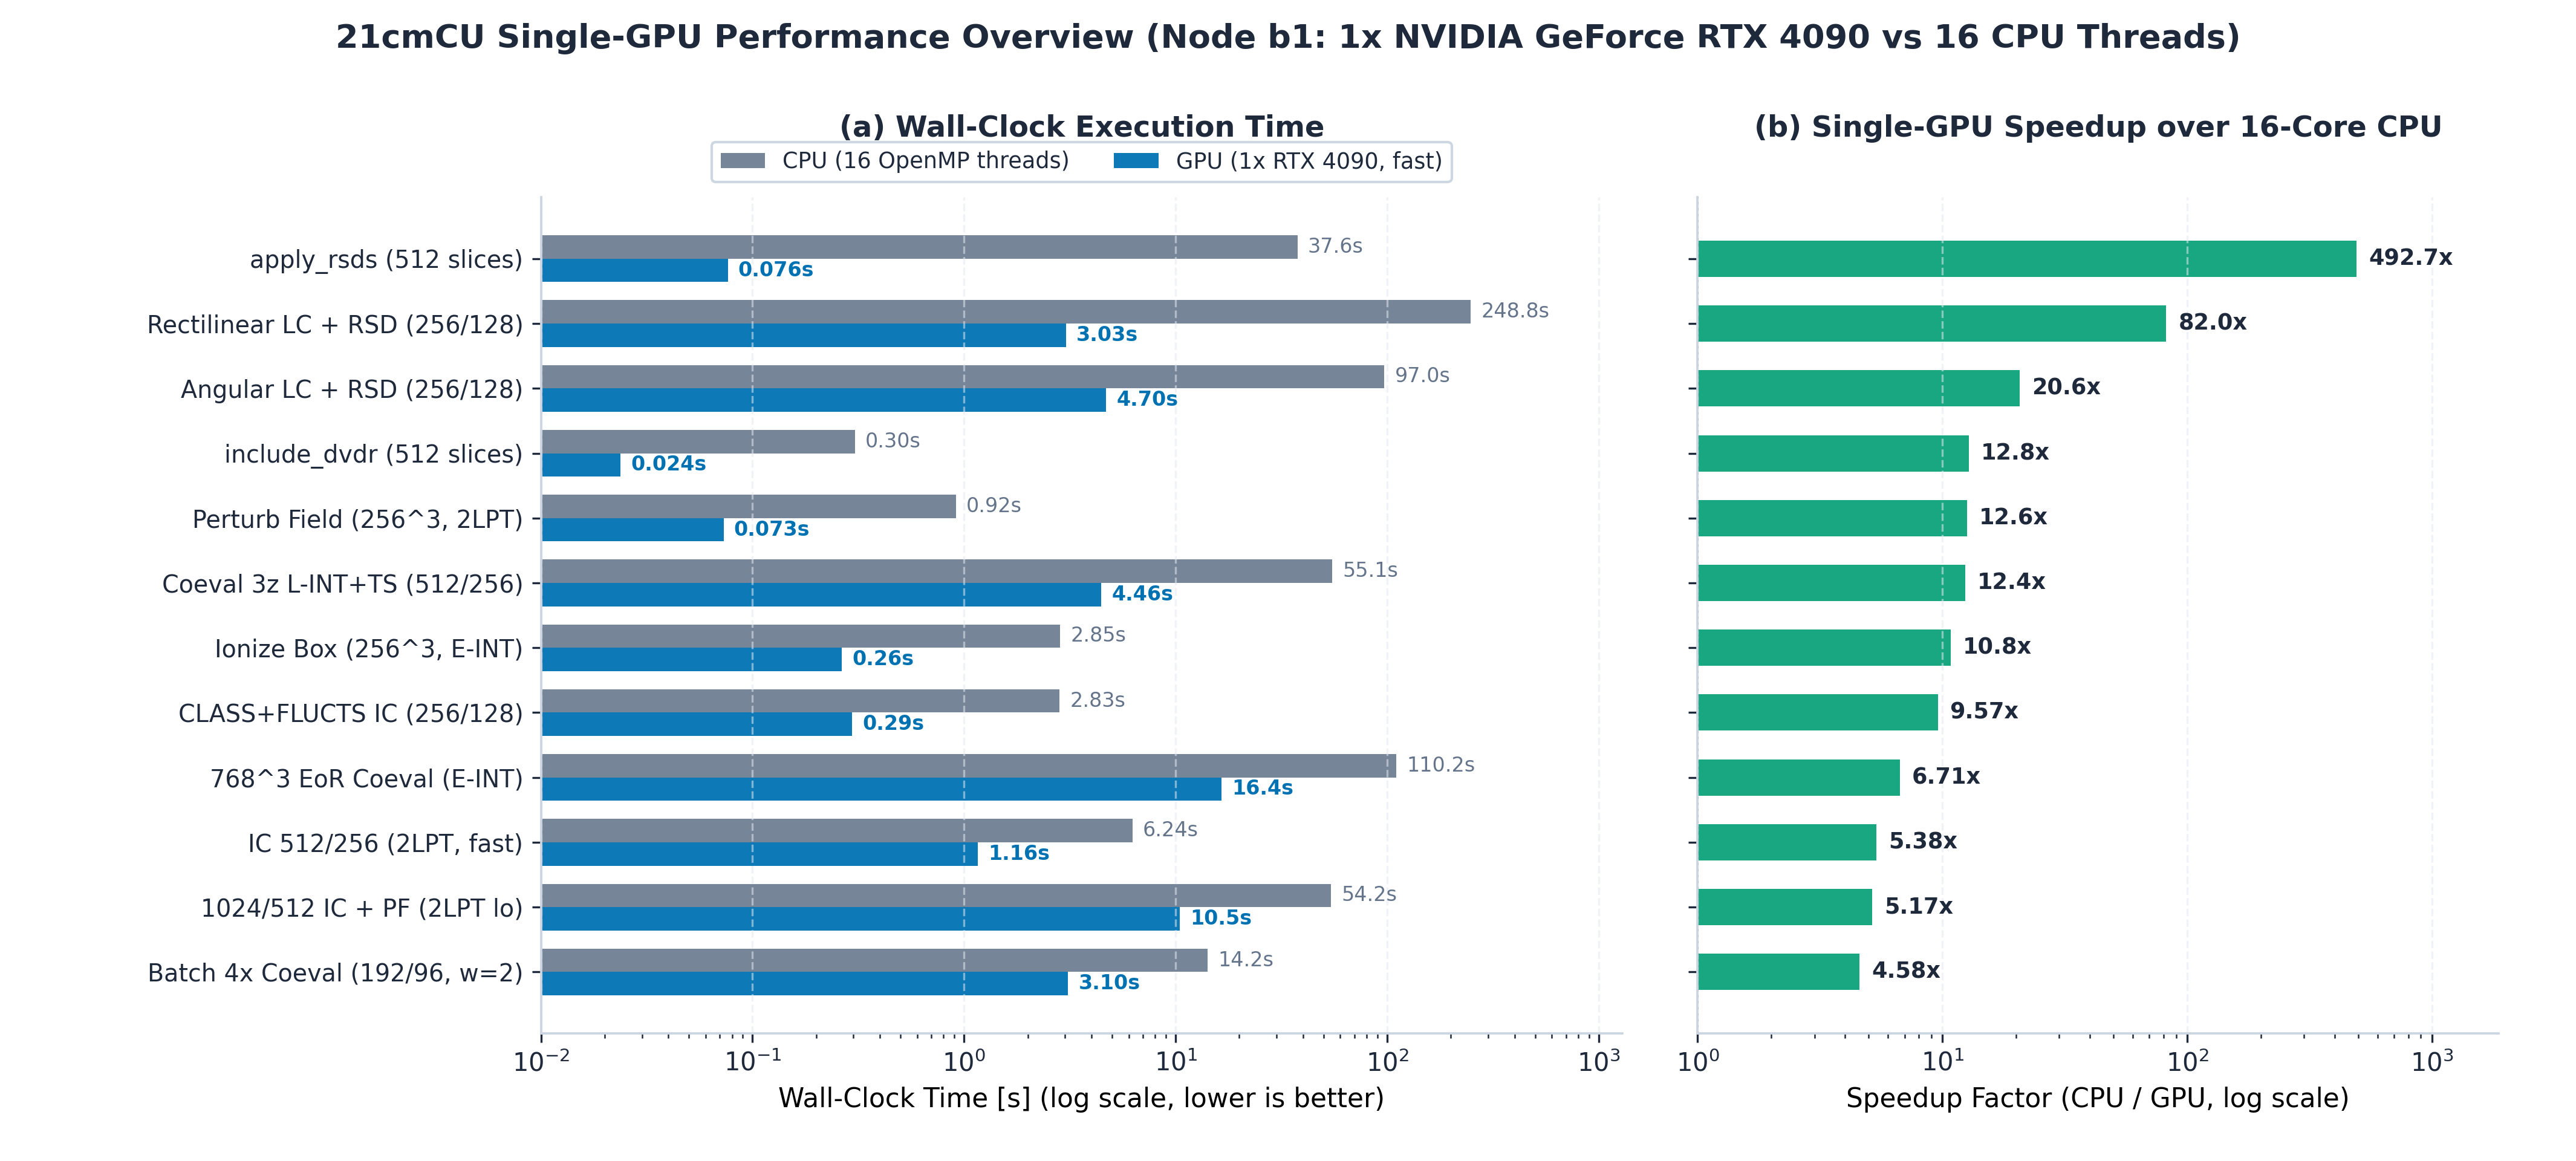
\includegraphics[width=\textwidth]{../figures/speedup_overview.png}
  \caption{Single-GPU (`1x RTX 4090`, \texttt{fast}) vs.\ 16-thread CPU wall-clock times (left) and speedup factors (right).}
  \label{fig:speedup}
\end{figure*}

\begin{table}[t]
\centering
\scriptsize
\begin{tabular}{@{}lrrr@{}}
\toprule
Workload & CPU 16T [s] & GPU [s] & Speedup \\
\midrule
\texttt{apply\_rsds} (512 slices) & 37.6455 & 0.0764 & \textbf{492.74$\times$} \\
Rectilinear LC ($z=6.5\text{--}11$) & 248.773 & 3.032 & \textbf{82.05$\times$} \\
Angular LC ($z=7.8\text{--}9.8$) & 97.018 & 4.698 & \textbf{20.65$\times$} \\
\texttt{include\_dvdr\_in\_tau21} & 0.305 & 0.0238 & \textbf{12.81$\times$} \\
Perturb Field (2LPT, $256^3$) & 0.915 & 0.073 & \textbf{12.58$\times$} \\
Coeval 3z (\texttt{L-INT+TS}, 512/256) & 55.079 & 4.456 & \textbf{12.36$\times$} \\
Ionize Box ($256^3$, \texttt{E-INT}) & 2.851 & 0.264 & \textbf{10.81$\times$} \\
\texttt{CLASS+FLUCTS} IC (256/128) & 2.827 & 0.295 & \textbf{9.57$\times$} \\
EoR Coeval ($768^3$, $z=7.0$) & 110.209 & 16.435 & \textbf{6.71$\times$} \\
2LPT IC (512/256) & 6.244 & 1.160 & \textbf{5.38$\times$} \\
IC + PF (1024/512, 2LPT lo) & 54.245 & 10.495 & \textbf{5.17$\times$} \\
Concurrent Batch ($4\times 192/96$) & 14.184 & 3.097 & \textbf{4.58$\times$} \\
\bottomrule
\end{tabular}
\caption{Single-GPU (\texttt{1x RTX 4090}, \texttt{fast}) vs.\ 16-core CPU baselines.}
\label{tab:single}
\end{table}

\begin{figure*}[t]
  \centering
  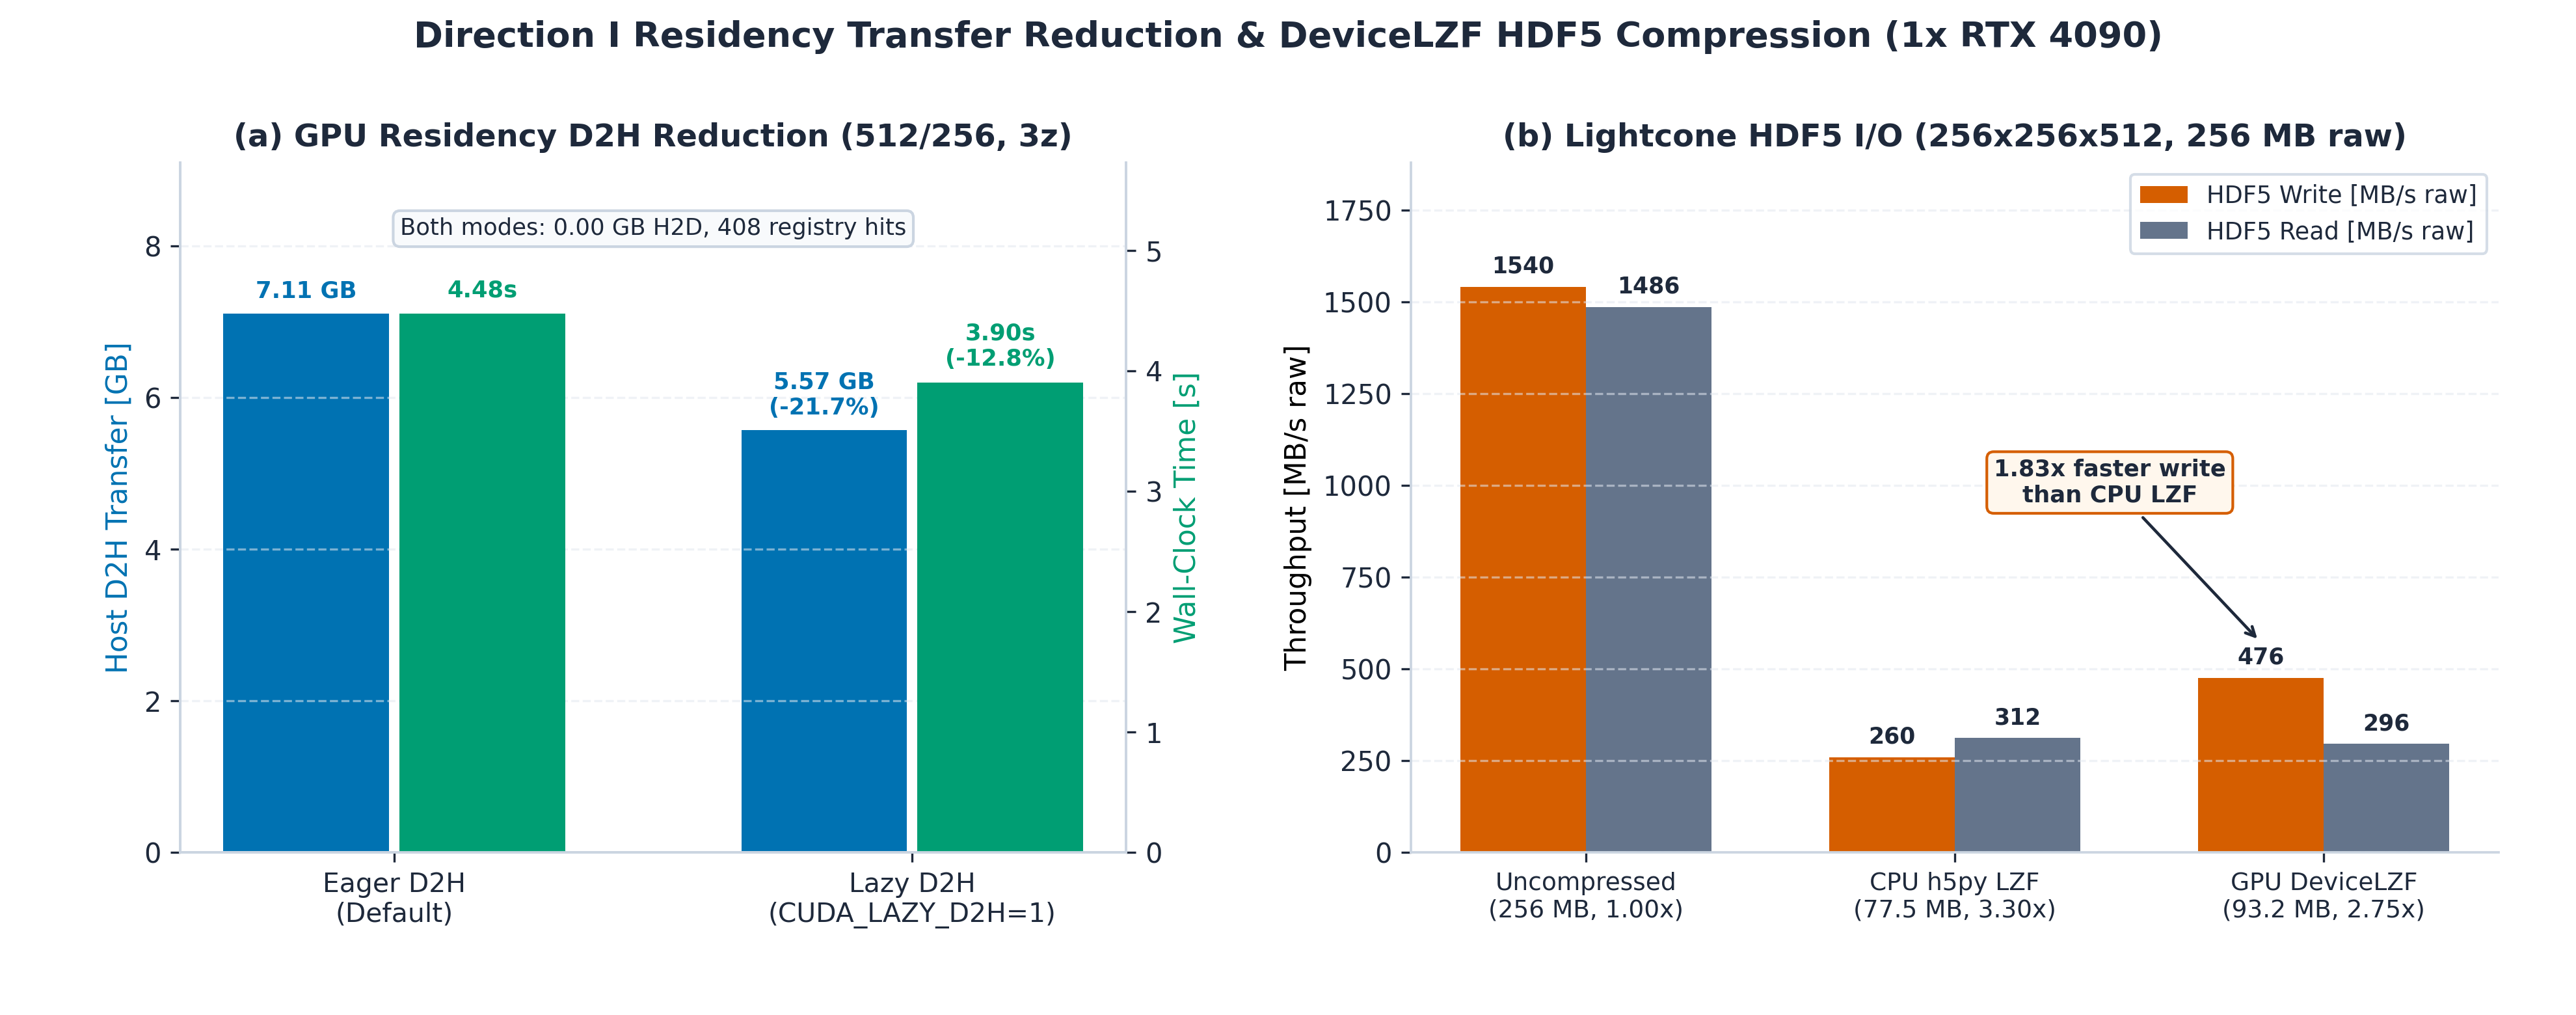
\includegraphics[width=\textwidth]{../figures/residency_and_io.png}
  \caption{Left: Opt-in \texttt{CUDA\_LAZY\_D2H} reduces D2H host traffic by 21.7\% and runtime by 12.8\% on 3z 512/256 coeval runs. Right: On-GPU \texttt{DeviceLZF} achieves 476.3\,MB/s HDF5 write throughput (1.83$\times$ CPU LZF).}
  \label{fig:io}
\end{figure*}

Under \texttt{CUDA\_LAZY\_D2H=True}, intermediate fields remain in the CUDA \texttt{DeviceFieldRegistry}, reducing D2H traffic on $512/256$ 3z runs from $7,113.54$\,MB to $5,570.04$\,MB ($-21.7\%$) and wall time from $4.477$\,s to $3.904$\,s ($-12.8\%$). Persistent \texttt{CLASS} \cite{Blas2011} \texttt{CosmoTables} caching cuts repeated initialization from $0.634$\,s cold to $0.311$\,ms in memory and $2.7$\,ms on disk, while \texttt{DeviceLZF} streams HDF5-compatible compressed chunks directly from GPU memory at $476.3$\,MB/s ($1.83\times$ CPU LZF).

\section{Multi-GPU Slab Decomposition and Single-Slab $2048^3$}
\begin{figure*}[t]
  \centering
  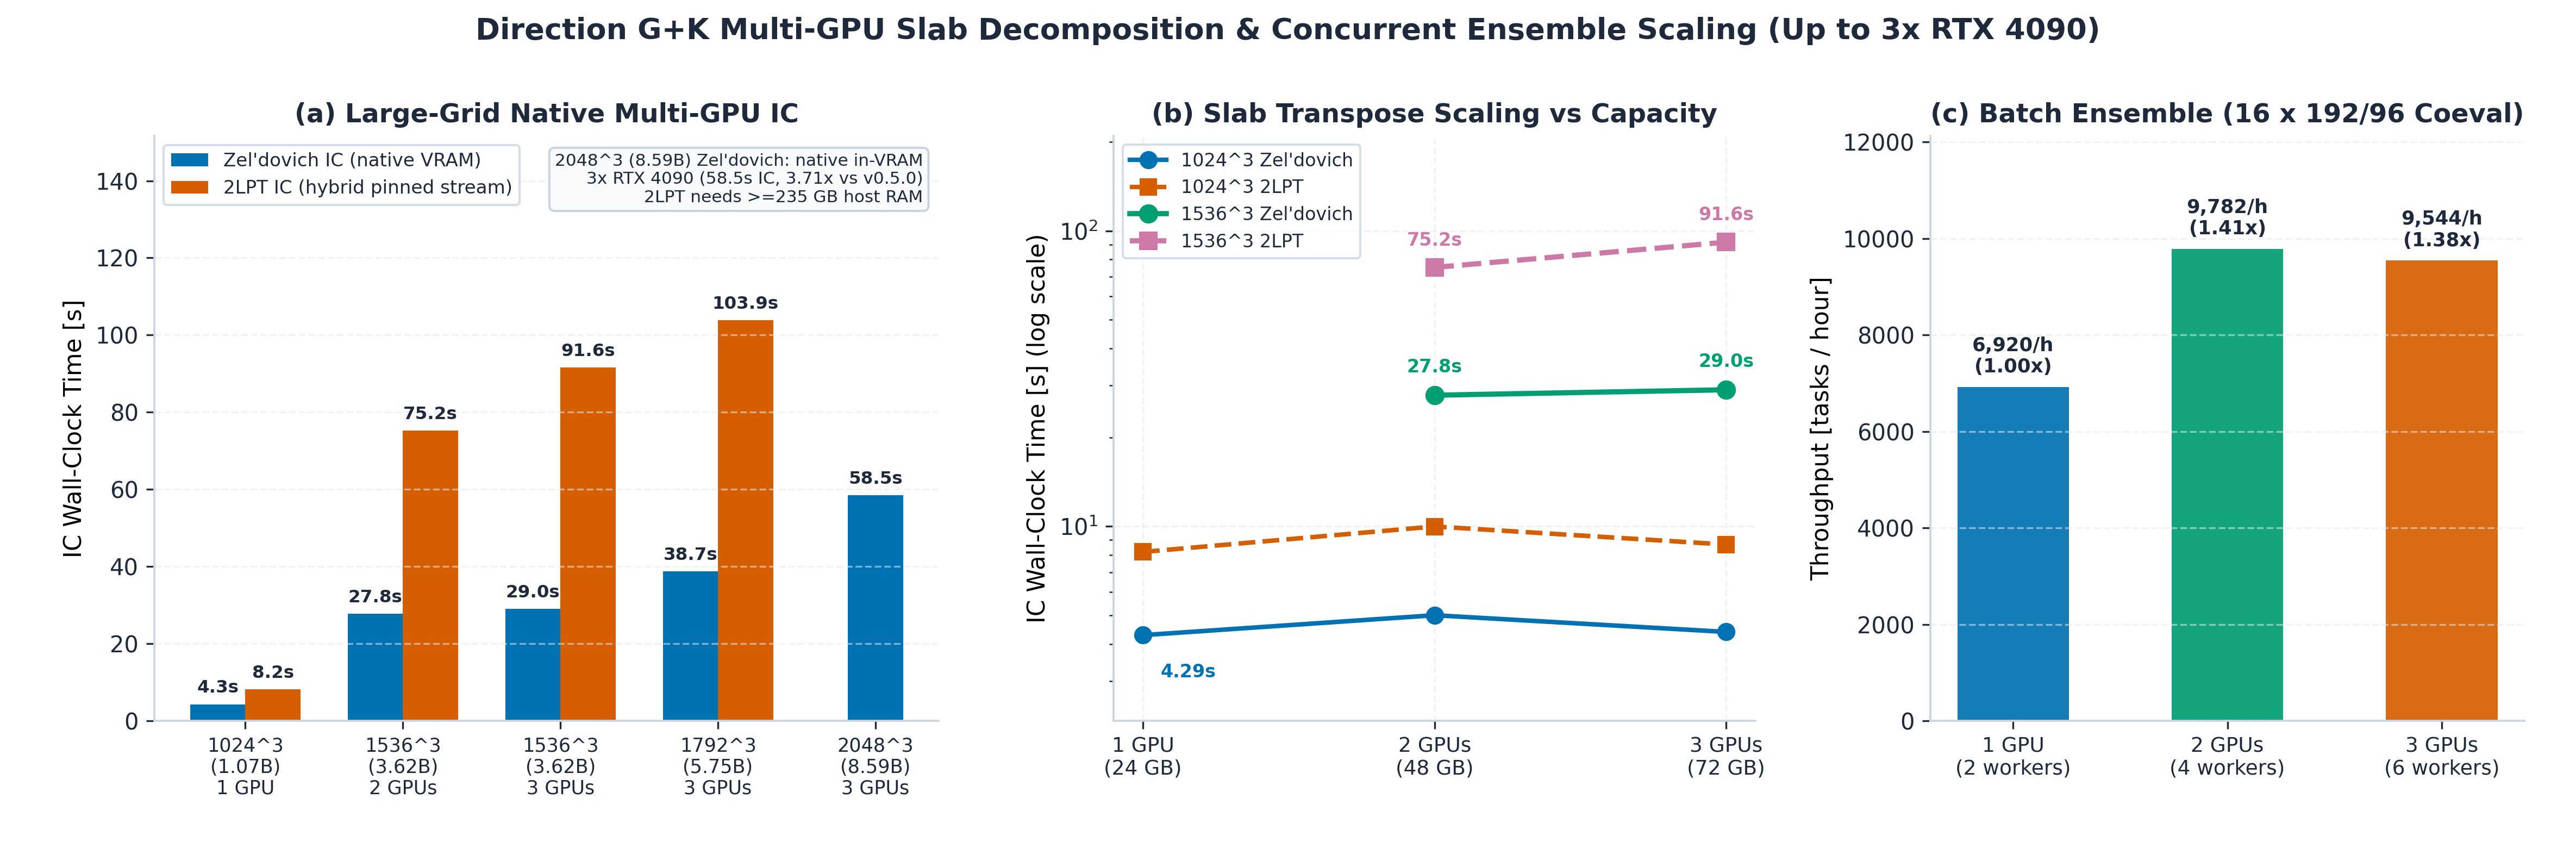
\includegraphics[width=\textwidth]{../figures/mgpu_scaling.png}
  \caption{Direction G+K multi-GPU slab decomposition up to $2048^3$ (left), scaling vs.\ capacity (middle), and multi-GPU \texttt{run\_batch} ensemble throughput (right).}
  \label{fig:mgpu}
\end{figure*}

To overcome the 24\,GB single-GPU limit above $1024^3$, \texttt{cuda\_mgpu.cu} splits 3D $(X,Y,Z/2+1)$ complex grids across $Y$-slabs with batched 2D R2C/C2R cuFFT, inter-GPU $X \leftrightarrow Y$ transposes, and batched 1D $Y$ C2C transforms. In v0.6.0 (Direction K), 64\,MiB pinned portable bounce buffers (\texttt{MgpuHostBounce}), \texttt{std::thread} sub-tiled transposes, zero-\texttt{h\_tmp\_ab} 2LPT streaming, and single-work-slab streaming enable native in-VRAM execution of $2048^3$ ($8.590\times 10^9$ voxels) Zel'dovich initial conditions across $3\times$ RTX 4090 in \textbf{58.467\,s} ($3.71\times$ faster than v0.5.0 host fallback), alongside $2.80\times$ speedup on $1536^3$ 2-GPU 2LPT ($75.231$\,s vs.\ $210.680$\,s) and $3.52\times$ on $1792^3$ 3-GPU 2LPT ($103.892$\,s vs.\ $365.663$\,s).

\section{SBI Data Pipeline, CLI, and Verification}
Directions L and M integrate Fourier-space horizon wedge filtering \cite{Parsons2012}, radiometer thermal noise, scrambled Sobol parameter sampling (\texttt{py21cmcu.observables}), HDF5-checkpointed resumable worker pools (\texttt{run\_batch}, up to $9,782.0$ tasks/h on $2\times$ RTX 4090), \texttt{doctor} hardware diagnostics, and the \texttt{21cmcu} CLI (\texttt{run}, \texttt{batch}, \texttt{doctor}, \texttt{bench}).

Across all 12 native GPU test suites (\texttt{test\_21cmcu\_phase0} through \texttt{phase6\_lm} and \texttt{test\_cuda\_phase1--3}, excluding \texttt{speed} micro-benchmarks), \texttt{21cmCU} passes \textbf{168/168 tests} on $3\times$ RTX 4090 (\texttt{cuda\_arch=sm\_89}) alongside \textbf{21/21} Phase 7--9 tests and \textbf{61/61} bit-exact C/OpenMP optimization parity tests.

\section{Higher-Order Topology, Online SBI, and Multi-Probe Forecasting (v0.7.0--v0.9.0)}
In \texttt{v0.7.0--v0.9.0}, \texttt{cuda\_analysis.cu} and \texttt{py21cmcu} extend the engine from 2-point power spectra to a complete multi-probe inference suite (Table~\ref{tab:t4v090}, reproducible via \texttt{benchmarks/reproduce\_v090\_tables.py}):
\begin{itemize}
  \item \textbf{Single-Pass Interferometer Mocks \& Zero-Copy DLPack}: \texttt{mock\_observation\_3d} combines UV coverage, PSF smoothing, channel response, horizon wedge filtering \cite{Parsons2012}, and radiometer thermal noise on $256^3$ cubes in $22.48\text{--}23.04$\,ms ($71.65\times\text{--}71.88\times$ vs.\ 16T CPU), while pure-\texttt{ctypes} \texttt{\_\_dlpack\_\_} views feed \texttt{OnlineSBIDataset} and warm \texttt{BatchPool} pipelines ($2.643\times$ on RTX 4090; $2.368\times$ on Tesla T4) with zero disk HDF5 writes.
  \item \textbf{Non-Gaussian \& Morphological Topology}: \texttt{bispectrum\_3d} ($26.64\times$ at $256^3$), Philox ray-traced \texttt{bubble\_size\_distribution\_mfp} ($62.53\times\text{--}72.87\times$) \cite{Mesinger2007}, and exact cubical-complex \texttt{minkowski\_functionals\_3d} ($8.28\times\text{--}8.48\times$) \cite{Schmalzing1997}.
  \item \textbf{Multi-Probe Cross-Correlations \& CRN Fisher}: Periodic 3D CIC gridding \texttt{p21\_cuda\_cic\_deposit\_3d} \cite{Hockney1988} with grid-stride loops for $>65535\times 256$ voxels accelerates $256^3$ 1M-particle gridding by \textbf{39.29$\times$} ($\max|\Delta\delta|=3.81\times 10^{-6}$), $21\text{cm} \times \text{galaxy}$ cross-power by \textbf{20.68$\times$} ($\max|\Delta r(k)|=2.91\times 10^{-8}$), and integrates with \texttt{ksz\_momentum\_map} \cite{Sunyaev1980} and Common-Random-Number \texttt{FisherForecaster}.
\end{itemize}

\begin{table*}[t]
\centering
\scriptsize
\begin{tabular}{@{}lrrrl@{}}
\toprule
Workload & Baseline [s] & T4 GPU [s] & Speedup & Parity / Notes \\
\midrule
Bispectrum 3D ($128^3$, equil.) & 0.8812 & 0.1420 & \textbf{6.21$\times$} & $\max|\Delta B|/|B|=1.31\times 10^{-6}$ \\
Bispectrum 3D ($256^3$, equil.) & 11.3274 & 0.4252 & \textbf{26.64$\times$} & $\max|\Delta B|/|B|=8.21\times 10^{-7}$ \\
MFP BSD ($128^3$, 200k rays) & 0.6947 & 0.0095 & \textbf{72.87$\times$} & $\langle R\rangle$ rel diff $3.66\times 10^{-3}$ \\
MFP BSD ($256^3$, 200k rays) & 2.3150 & 0.0370 & \textbf{62.53$\times$} & $\langle R\rangle$ rel diff $5.0\times 10^{-4}$ \\
Minkowski ($128^3$, 15 thresh.) & 0.2960 & 0.0357 & \textbf{8.28$\times$} & Exact Euler $\chi$ \\
Minkowski ($256^3$, 15 thresh.) & 3.0784 & 0.3632 & \textbf{8.48$\times$} & Exact Euler $\chi$ \\
\texttt{cic\_deposit\_3d} ($256^3$, 1M) & 1.4336 & 0.0365 & \textbf{39.29$\times$} & $\max|\Delta\delta|=3.81\times 10^{-6}$ \\
\texttt{cross\_power\_21cm\_galaxy} ($256^3$, 1M) & 4.8076 & 0.2324 & \textbf{20.68$\times$} & $\max|\Delta r(k)|=2.91\times 10^{-8}$ \\
\texttt{BatchPool} Warm ($4\times 2$, T4) & 26.7845 (cold) & 11.3101 (warm) & \textbf{2.368$\times$} & Round 4: 1.2729\,s; 1 PID \\
\bottomrule
\end{tabular}

\caption{Verified \texttt{v0.9.0} higher-order topology, warm \texttt{BatchPool}, and multi-probe CIC / cross-power benchmarks on Google Colab Tesla T4 (\texttt{benchmarks/results\_t4\_v090.json}).}
\label{tab:t4v090}
\end{table*}

\bibliographystyle{unsrt}
\bibliography{refs}
\end{document}
